\documentclass[12pt,a4paper]{book}
\usepackage[utf8]{inputenc}
\usepackage[spanish]{babel}
\usepackage{url}
\usepackage{times}
\usepackage{graphicx}
\usepackage{float}  %% H para posicionar figuras
\usepackage[nottoc, notlot, notlof, notindex]{tocbibind} %% Opciones de índice
\usepackage{latexsym}  %% Logo LaTeX
\usepackage[left=2cm,right=2cm,top=2cm,bottom=2cm]{geometry}

\title{Práctica 8.\\ Localización}
\author{Sandra Gómez Gálvez & Sergio Casado López}

\renewcommand{\baselinestretch}{1.5}  %% Interlineado

\begin{document}

%%%%PORTADA:
\begin{titlepage}
\begin{center}
\begin{tabular}[c]{c c}


\includegraphics[scale=0.25]{urjc.png} 
\begin{tabular}[b]{l}
\Huge
\textsf{UNIVERSIDAD} \\
\Huge
\textsf{REY JUAN CARLOS} \\
\end{tabular}

\end{tabular}
\vspace{3cm}

\Large
INGENIERÍA DEL SOFTWARE Y MATEMÁTICAS

\vspace{0.4cm}

\large
Curso Académico 2018/2019

\vspace{0.8cm}



\vspace{2.5cm}

\LARGE
PRÁCTICA 8 - Localización

\vspace{4cm}

\large
Autores : Sandra Gómez Gálvez y Sergio Casado López\\
\end{center}
\end{titlepage}
\newpage
\mbox{}
\thispagestyle{empty} % para que no se numere esta pagina
% ÍNDICE %
\tableofcontents 
%%%%%%%%%%%%%%%%%%%%%%%%%%%%%%%%%%%
%%%%%%%%%%%

\chapter{Localización}
\label{sec:af} % etiqueta para poder referenciar luego en el texto con ~\ref{sec:r2}
\pagenumbering{arabic}
Resolveremos el problema\textit{ 1-centro } del test  \textit{"phub  50  5  5.txt"} 
para ello utilizaremos el \textit{Algoritmo 1-centro, } cual tiene el siguiente pseudocódigo: 
\begin{figure}[H]

\includegraphics[scale=0.5]{Captura1.png} 
\label{fig:ps1}
\end{figure}
\begin{figure}[H]
\centering
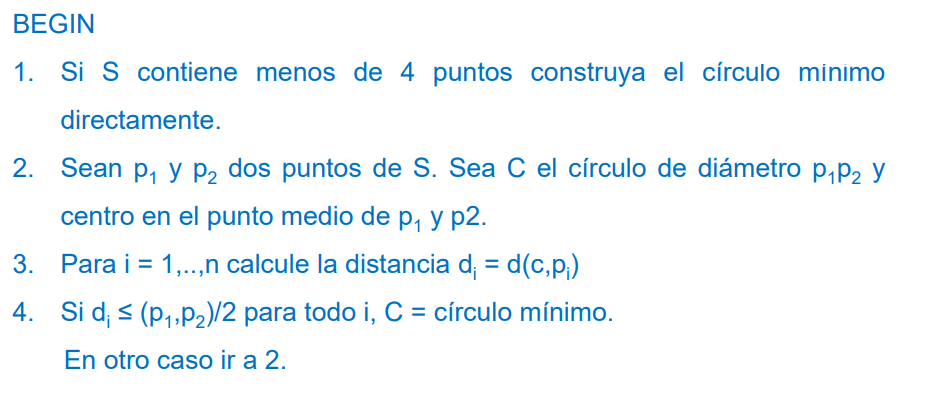
\includegraphics[scale=0.5]{Captura2.png} 
\label{fig:ps2}
\end{figure}
\begin{figure}[H]
\centering
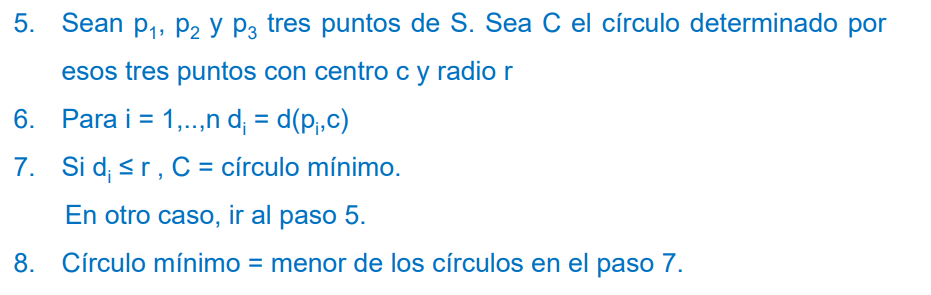
\includegraphics[scale=0.5]{Captura3.png} 
\caption{Pseudocódigo Algoritmo 1-centro}
\label{fig:ps3}
\end{figure}
Por tanto, en R, para codificarlo tendremos 4 funciones: \textit{alg1Centro, distancia, puntoMedio y dibujar.}
\section{Funciones}
\subsection{Función alg1Centro}
Comenzaremos con la función \textbf{\textit{alg1Centro:}}
\\Esta función comienza con una sentencia if/else, dónde en el if se evaluarán todos los conjuntos de puntos menores de 4 puntos, y en el else los conjuntos de 4 puntos o más. 

\subsubsection{if}
En el  if: 
\begin{figure}[H]
\centering

\includegraphics[scale=0.75]{Captura4.png} 
\label{fig:pif1}
\end{figure}
\begin{figure}[H]
\centering
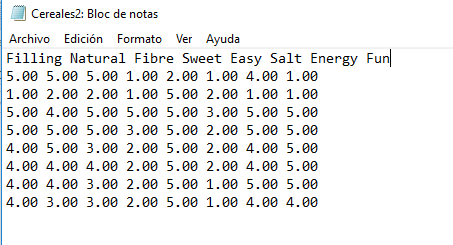
\includegraphics[scale=0.75]{Captura5.png} 
\label{fig:pif2}
\end{figure}
\begin{figure}[H]
\centering
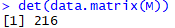
\includegraphics[scale=0.75]{Captura6.png} 
\caption{Algoritmo 1-centro - Parte if de la estructura if/else}
\label{fig:pif3}
\end{figure}
Como podemos ver, dentro del if, encontramos otra sentencia if/else anidada, dónde se evaluará si el conjunto de puntos está compuesto por un solo punto, dos puntos o tres puntos. 
\\Para el caso igual a un punto, el cálculo del centro mínimo es ese mismo punto y el radio mínimo es, por tanto, cero. 
\\Para el caso igual a dos puntos, el centro mínimo es el punto medio entre ambos puntos y el radio mínimo la distancia entre ambos puntos entre 2. 
\\Para el caso igual a tres puntos, el centro y radio mínimos lo calcularemos de la siguiente manera: 
\\En primer lugar, sabemos que la ecuación general de una circunferencia  $ x^{2}+y^{2}+Ax+Bx+C=0 $  tiene 3 parámetros a determinar que son  A, B y C . 
\\Mediante los 3 puntos que entran en la función, calcularemos A, B, y C.
\\Por lo tanto, realizaremos un sistema de 3 ecuaciones para determinar los 3 parámetros. 
\\Si nuestra matriz asociada a la parte izquierda de nuestro sistema tiene un determinante distinto de 0, entonces, será invertible y podremos proceder a solucionar el sistema. Posteriormente, sacaremos el radio mínimo con la fórmula: $ radio = (\sqrt(A^{2} + B^{2}- 4*C))/ 2 $ , y el centro mínimo: $ centrox = -(A/2); centroy = -(B/2) --> centroMin = (centrox, centroy) $ . 
\\En el caso de que el determinante de nuestra función sea igual a cero, tendremos que ver subcasos: 
\\ - Primero veremos si los puntos están alineados en vertical, en ese caso cogeremos el punto que esté más arriba en el eje y y el otro punto que se encuentre más abajo en el eje y.  Y con ellos procederemos a sacar el centro y el radio mínimos como en el caso de un conjunto de dos puntos.
\\ - Si los puntos no están alineados en el eje vertical, sacaremos 2 puntos: el que esté más a la izquierda y el que esté más a la derecha.   Y con ellos procederemos a sacar el centro y el radio mínimos como en el caso de un conjunto de dos puntos.
\subsubsection{else}
En el  else:
\begin{figure}[H]
\centering
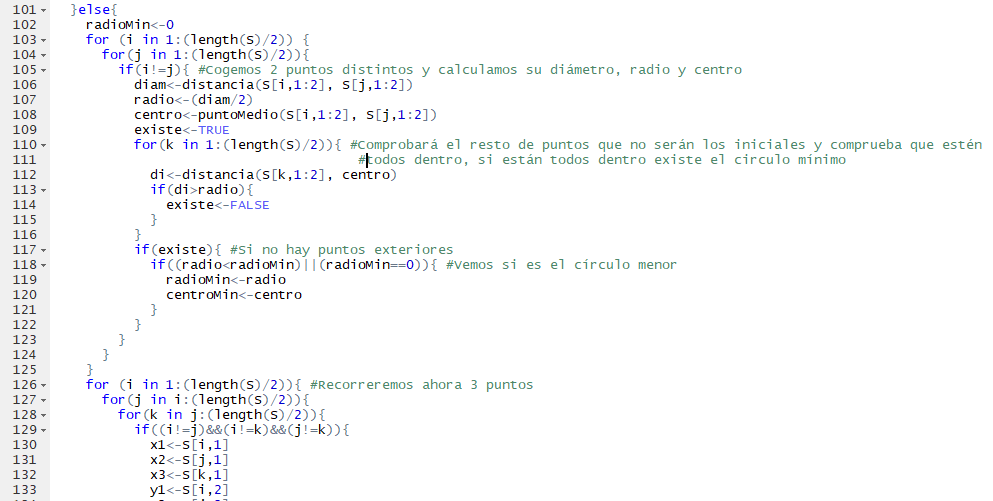
\includegraphics[scale=0.6]{Captura7.png} 
\label{fig:pelse1}
\end{figure}
\begin{figure}[H]
\centering
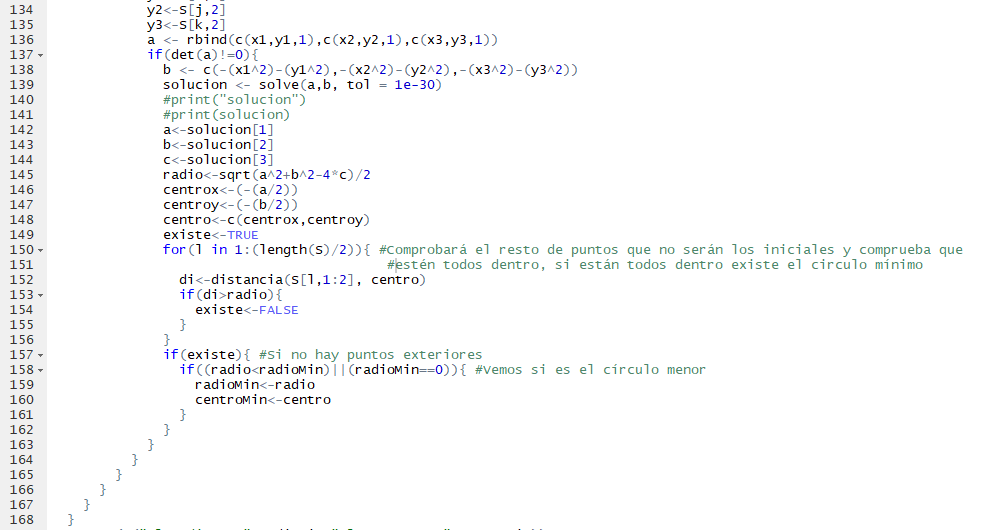
\includegraphics[scale=0.6]{Captura8.png} 
\caption{Algoritmo 1-centro - Parte else de la estructura if/else}
\label{fig:pelse2}
\end{figure}
En esta parte encontraremos los algoritmos voraces: 
\\ -1) Primero cogeremos 2 puntos distintos y calcularemos su diámetro, radio y centro. Después comprueba si existe el círculo mínimo, es decir, si todos los demás puntos están dentro. Y finalmente, si el círculo mínimo existe, instaura el radio y centro como radio mínimo y centro mínimo respectivamente. 
\\ -2) Ahora, recorreremos 3 puntos distintos, para ello, como anteriormente: En primer lugar, sabemos que la ecuación general de una circunferencia  $ x^{2}+y^{2}+Ax+Bx+C=0 $  tiene 3 parámetros a determinar que son  A, B y C . Mediante los 3 puntos que entran en la función, calcularemos A, B, y C. Por lo tanto, realizaremos un sistema de 3 ecuaciones para determinar los 3 parámetros. Si nuestra matriz asociada a la parte izquierda de nuestro sistema tiene un determinante distinto de 0, entonces, será invertible y podremos proceder a solucionar el sistema. Posteriormente, sacaremos el radio mínimo con la fórmula: $ radio = (\sqrt(A^{2} + B^{2}- 4*C))/ 2 $ , y el centro mínimo: $ centrox = -(A/2); centroy = -(B/2) --> centroMin = (centrox, centroy) $ . Finalmente, comprobará que el resto de puntos no sean los iniciales y que estén todos dentro, si están todos dentro existe el círculo mínimo. Si existe el círculo mínimo, instaura el radio y centro como radio mínimo y centro mínimo respectivamente. 
\subsubsection{return}
\begin{figure}[H]
\centering
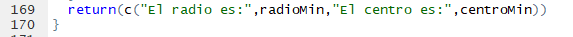
\includegraphics[scale=1]{Captura9.png} 
\caption{Algoritmo 1-centro - return}
\label{fig:pelse2}
\end{figure}
Finalmente, la función devuelve un vector donde en la posición 1 devolverá el String "El radio es:", en la posición dos devolverá radioMin, en la posición tres el String "El centro es: " y en la última posición el centroMin.
\\Finalizando así la función alg1Centro
\subsection{Función distancia}
\begin{figure}[H]
\centering
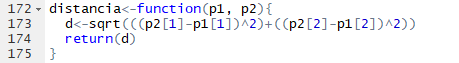
\includegraphics[scale=1]{Captura10.png} 
\caption{Función distancia}
\label{fig:fd}
\end{figure}
Está función calcula la distancia que hay entre dos puntos de la siguiente manera: 
\\$ distancia = \sqrt{(x2-x1)^2 + (y2-y1)^2} $
\subsection{Función puntoMedio}
\begin{figure}[H]
\centering
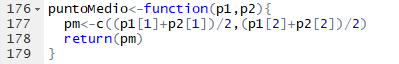
\includegraphics[scale=1]{Captura11.png} 
\caption{Función Punto Medio}
\label{fig:fpm}
\end{figure}
Está función calcula el punto medio entre dos puntos, de la siguiente manera: 
\\$ puntoMedio = ( (x1+x2)/2, (y1+y2)/2 )$
\subsection{Función dibujar}
\begin{figure}[H]
\centering
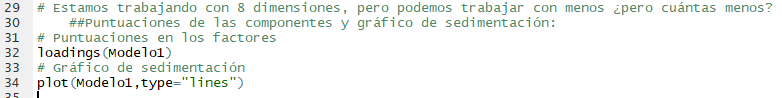
\includegraphics[scale=0.6]{Captura12.png} 
\caption{Función dibujar}
\label{fig:fdb}
\end{figure}
Está función dibuja el círculo mínimo que cubre todos los puntos. 
\section{Resolución del problema}
\begin{figure}[H]
\centering
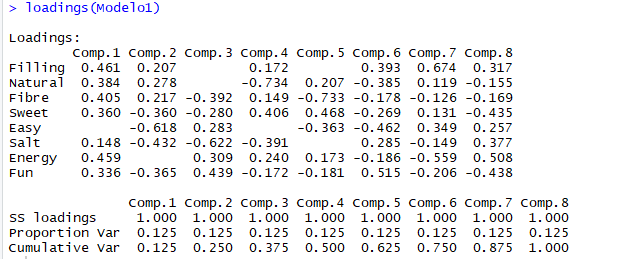
\includegraphics[scale=0.6]{Captura13.png} 
\caption{Resolución del problema - Parte 1}
\label{fig:rs}
\end{figure}
Para resolver el problema, leeremos los datos y los meteremos en una matriz, cogiendo solo las dos primeras columnas, que corresponden a cada par de puntos x e y. 
\begin{figure}[H]
\centering
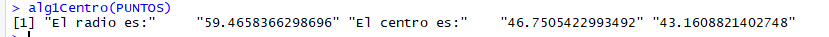
\includegraphics[scale=0.75]{Captura14.png} 
\caption{Resolución del problema - Parte 2}
\label{fig:rs2}
\end{figure}
A continuación, llamamos por consola a la función alg1Centro introduciéndole la matriz de PUNTOS. 
\begin{figure}[H]
\centering
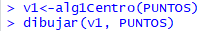
\includegraphics[scale=1]{Captura15.png} 
\caption{Resolución del problema - Parte 3}
\label{fig:rs3}
\end{figure}
Y finalmente, llamando por consola al alg1Centro y a dibujar, obtenemos: 
\begin{figure}[H]
\centering
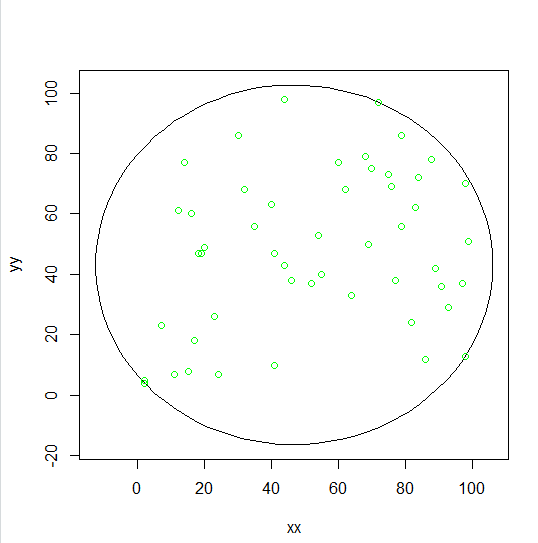
\includegraphics[scale=1]{Captura16.png} 
\caption{Resolución del problema - Parte 4 - Círculo Mínimo Final}
\label{fig:rs4}
\end{figure}
Que como podemos comprobar es el círculo mínimo posible. 
\section{Anexo}
Como nuestro problema nos da más de 3 puntos, no podemos comprobar si los otros casos de nuestro algoritmo están bien. 
Por tanto, los comprobaremos: 
\\Para el caso igual a un punto, solo es ese punto.
\\Para el caso igual a dos puntos: 
\begin{figure}[H]
\centering
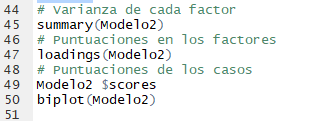
\includegraphics[scale=1]{Captura17.png} 
\caption{Círculo Mínimo 2 puntos}
\label{fig:cm2p}
\end{figure}
\begin{figure}[H]
\centering
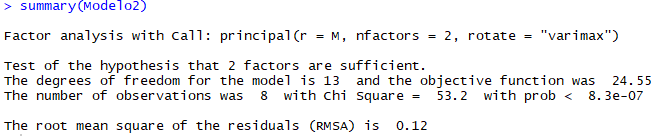
\includegraphics[scale=1]{Captura18.png} 
\caption{Círculo Mínimo 2 puntos}
\label{fig:cm2ps}
\end{figure}
Para el caso igual a tres puntos: 
\begin{figure}[H]
\centering
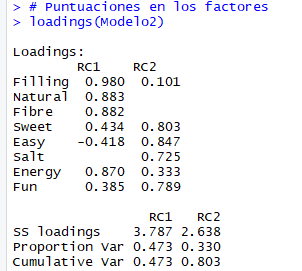
\includegraphics[scale=1]{Captura19.png} 
\caption{Círculo Mínimo 3 puntos}
\label{fig:cm3p}
\end{figure}
\begin{figure}[H]
\centering
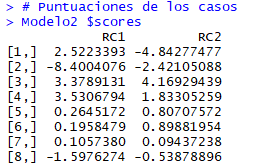
\includegraphics[scale=1]{Captura20.png} 
\caption{Círculo Mínimo 3 puntos}
\label{fig:cm3ps}
\end{figure}
Si encontramos los 3 puntos alineados horizontalmente: 
\begin{figure}[H]
\centering
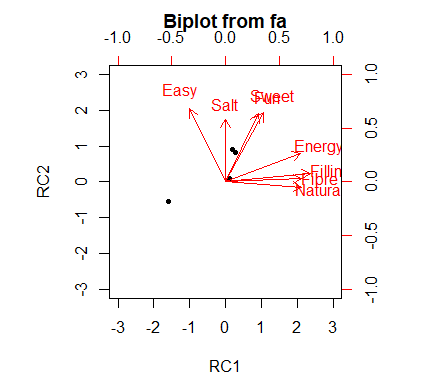
\includegraphics[scale=1]{Captura21.png} 
\caption{Círculo Mínimo 3 puntos horizontal}
\label{fig:cm3ph}
\end{figure}
\begin{figure}[H]
\centering

\includegraphics[scale=1]{Captura22.png} 
\caption{Círculo Mínimo 3 horizontal}
\label{fig:cm3psh}
\end{figure}
Si encontramos los 3 puntos alineados verticalmente: 
\begin{figure}[H]
\centering
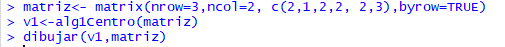
\includegraphics[scale=1]{Captura23.png} 
\caption{Círculo Mínimo 3 puntos vertical}
\label{fig:cm3pv}
\end{figure}
\begin{figure}[H]
\centering
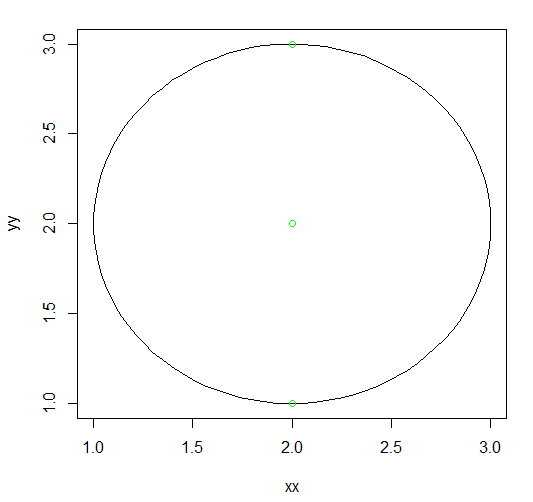
\includegraphics[scale=1]{Captura24.png} 
\caption{Círculo Mínimo 3 vertical}
\label{fig:cm3psv}
\end{figure}
Observamos como para todos los casos nuestro algoritmo 1-centro calcula correctamente el círculo mínimo. 
\end{document}
